From the linearised equation $x^2=\frac{2mg}{k}\cdot h_0$ , we can plot $x^2$ against $h_0$ and obtain a linear line passing through the origin with an expected gradient of $\frac{2mg}{k}$. By comparing this against a directly calculated value of $\frac{2mg}{k}$ through direct measurement and literature value, we can determine the experimental error.
\FloatBarrier
\begin{figure}[!htb]
    \begin{center}
        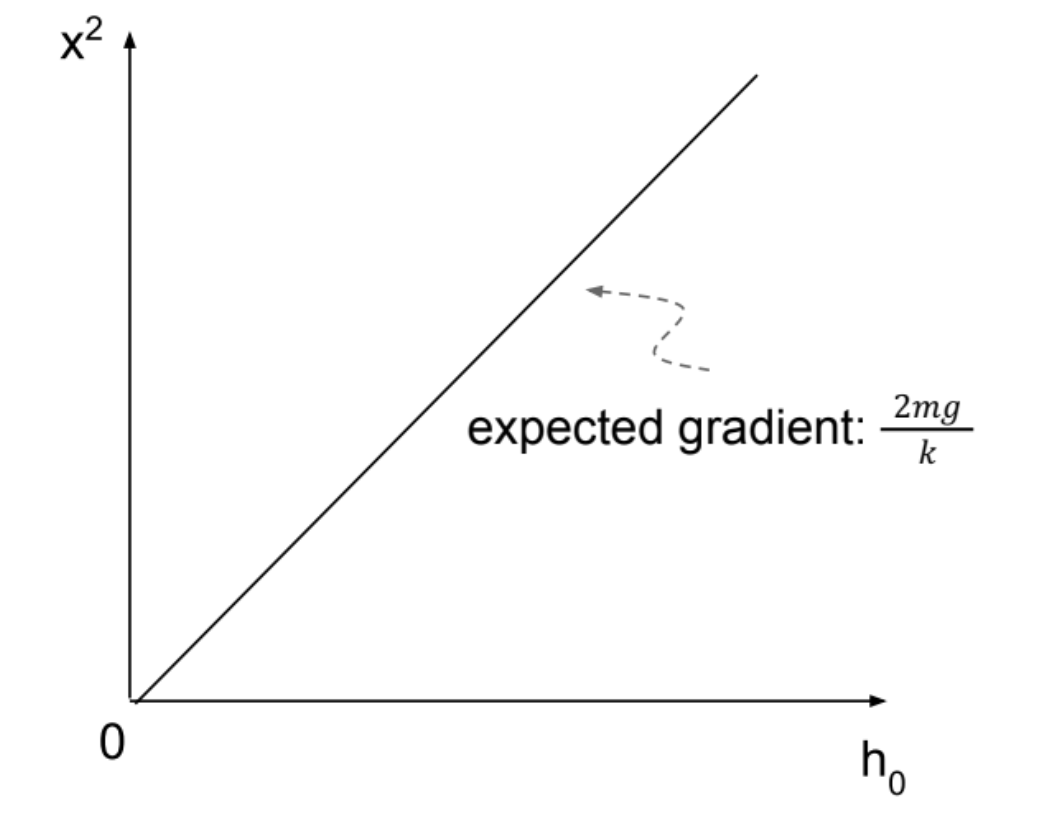
\includegraphics[width = 200px]{grad.png}
    \end{center}
\end{figure}
\FloatBarrier